\section{Bisection and Newton-Raphson method for finding roots}

\subsection{Bisection method}

We will use the bisection method to find when $y_p(\phi)=0$ for a given tolerance $\epsilon$. 
The requirement for the bisection method is that the function in question is continuous on the closed interval $[a,b]$\footnote{\href{https://mathworld.wolfram.com/Bisection.html}{Bisection method - Wolfram MathWorld}}, so the roots of $y_p(\phi)$ can be found. The roots of $w\,'(\phi)$ will be found using the Newton's method later.

\subsection{Newton-Raphson method}

In Eq. 40 from the presentation, $w_p\,'(\phi)$ was not expressed in terms of $\beta$, 
so the following expression will be used:

\begin{equation}
    w_p\,'(\phi)=\frac{2(\sin^2(2\phi+\pi/2)-3)\sin(2\phi+\pi/2)}{(3\pi+8)\beta^2\sin^3(2\phi+\pi/2)}
    -\frac{\cos(2\phi+\pi/2)\left(1-\frac{4}{(3\pi+8)\beta^2}(3\phi+2)\right)}{r_0\sin^3(2\phi+\pi/2)}
\end{equation}

This method cannot be used to solve for the root of $y_p(\phi)$ because although the function exists in the domain $\phi\in[0,\pi/4)$,
$\lim_{\phi\to 0^+}y_p\,'(\phi)$ and $\lim_{\phi\to \pi/4^-}y_p\,'(\phi)$ do not exist, so the function is not differentiable on the entire interval\footnote{\href{http://amsi.org.au/ESA_Senior_Years/SeniorTopic3/3j/3j_2content_2.html}{Newton's method}}.

From observing the graph of $y_p(\phi)$ on Page 6, this is confirmed visually. Since the endpoints of $y_p(\phi)$ on this interval are its two roots,
they cannot be found through this method. The bisection method works, however, since the only requirement is continuity of $y_p(\phi)$ on the interval.

\begin{figure}[H]
    \centering
    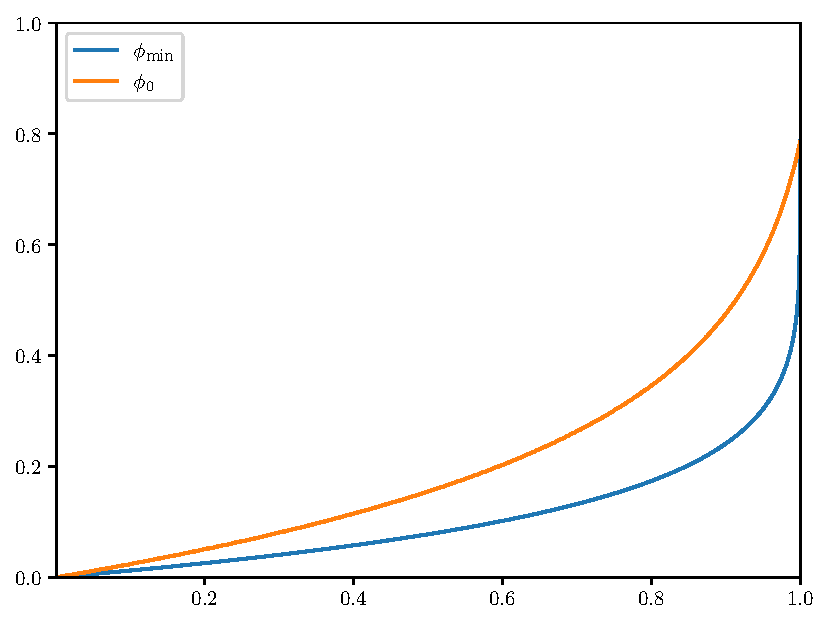
\includegraphics[]{plots/phi-functions.pdf}
    \caption{A plot of $\phi_\mathrm{min}$ and $\phi_0$ vs $\delta$}\label{phifig}
\end{figure}

The code used to implement both algorithms is located \href{https://gist.github.com/sidnb13/d715682a9915ec4cf49d66ceb2e54855}{here}.

\section{Curve fitting}

\subsection{Objective}

The least-squared method of curve fitting\footnote{\href{https://www.dam.brown.edu/people/alcyew/handouts/leastsq.pdf}{Curve fitting: least squares methods}} was used to generate the closed-form equations $\phi_0(\delta)$ and $\phi_\mathrm{min}(\delta)$.

The approach is to define an error function $E(\phi)=\sqrt{\frac{1}{n}\sum_{i=1}^n(\phi_i-\phi(\delta_i))^2}$ that represents the RMS error between the fitted curve and original data. $n$ is the number of data points in the set $\{(\delta_1,\phi_1),\ldots,(\delta_n,\phi_n)\}$ and $\phi(\delta)$ represents the fitted curve.
Because a polynomial curve is desired, the coefficients of the terms in $\delta(\phi)$ belong to $\vec c\in \mathbb{R}^{k+1}$, so there are $k+1$ coefficients in the fitted polynomial. Since $\phi(\delta;\vec{c})$, $E:\mathbb{R}^{k+1}\to \mathbb{R};\vec{c}$. The objective is then to find a $\vec{c}$ which minimizes $E(\vec{c})$. Similarly, each $\phi(\delta_i)$ becomes a function of $\vec{c}$.

Minimizing $E(\vec{c})=\sqrt{\frac{1}{n}\sum_{i=1}^n(\phi_i-\phi(\delta_i))^2}$ is the same as minimizing $E_1(\vec{c})=\sum_{i=1}^n(\phi_i-\phi(\delta_i))^2$, so the next step is to solve

\begin{gather}
    \frac{\partial E_1}{\partial c_j}=2\sum_{i=1}^n(\phi_i-\phi(\delta_i)) \frac{\partial \phi(\delta_i)}{\partial c_j}=0\\
    \sum_{i=1}^n\frac{\partial \phi(\delta_i)}{\partial c_j}\phi_i=\sum_{i=1}^n\frac{\partial \phi(\delta_i)}{\partial c_j}\phi(\delta_i)\\
    \sum_{i=1}^n \delta_i^{j-1}\phi_i=\sum_{i=1}^n c_j\delta_i^{2j-1}+\ldots+c_1\delta_i^{j-1}=\sum_{\ell=1}^j\sum_{i=1}^n c_{j-\ell+1}\delta_i^{2j-\ell-1}
\end{gather}

where $j=1,\ldots,k+1$ and the polynomial is of degree $k$.

A vectorized implementation yields

\begin{equation}
    \begin{bmatrix}\sum_{i=1}^n \delta_i^k\phi_i\\\vdots\\\sum_{i=1}^n \delta_i^1\phi_i\end{bmatrix}
    =\begin{bmatrix}\sum_{i=1}^n\delta_i^{2k}&\cdots&\sum_{i=1}^n\delta_i^{k}\\\vdots&\ddots&\vdots\\\sum_{i=1}^n \delta_i^{k}&\cdots&\sum_{i=1}^n\end{bmatrix}
    \begin{bmatrix}c_{k+1}\\\vdots\\c_1\end{bmatrix}
    =\begin{bmatrix}\sum_{i=1}^nc_{k+1}\delta_i^{2k}&\cdots&\sum_{i=1}^nc_1\delta_i^{k}\\\vdots&\ddots&\vdots\\\sum_{i=1}^n c_{k+1}\delta_i^{k}&\cdots&\sum_{i=1}^nc_1\end{bmatrix}\\
\end{equation}

\begin{equation}
    \vec{b}=A\vec{c}
\end{equation}

The matrix-vector equation $A\vec{c}=\vec{b}$ can then be solved for $\vec{c}$ using an optimized linear algebra library, and the resulting coefficients used to generate a function $\phi(\delta)$.

\begin{figure}[H]
    \centering
    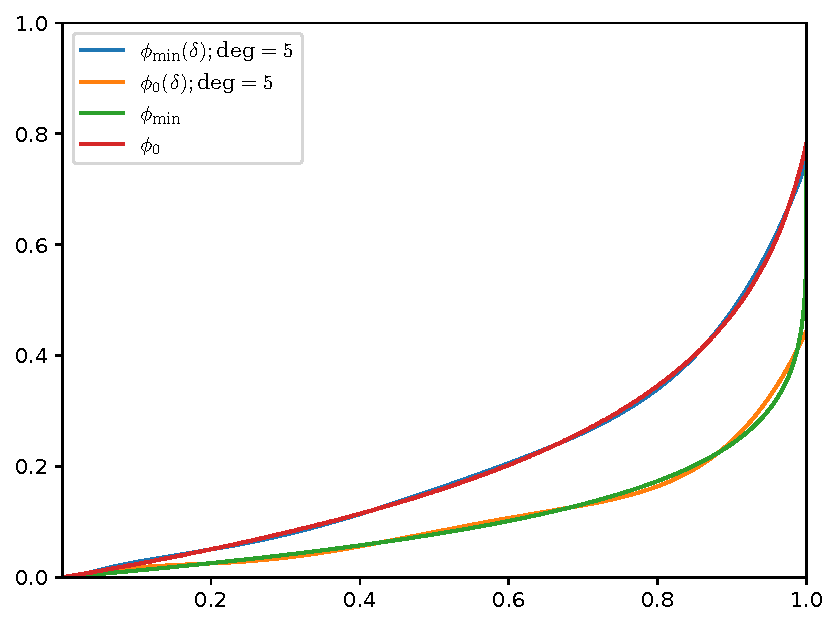
\includegraphics[]{plots/phi-curve-fit-poly.pdf}
    \caption{Using degree 5 polynomials to approximate $\phi_0(\delta)$ and $\phi_\mathrm{min}(\delta)$}\label{polyerror}
\end{figure}

A better approximation is desired since even with degree 5, a polynomial approximation cannot fit well to the smooth curves of $\phi_0$ and $\phi_\mathrm{min}$. This is evidenced by the Runge effect visible in the error plot of Figure \ref{polyerror}.

\subsection{Attempted approximation using Chebyshev polynomial interpolation}

The Chebyshev polynomial approximations resulted in a more pronounced Runge effect, as depicted below.

\begin{figure}[H]
    \centering
    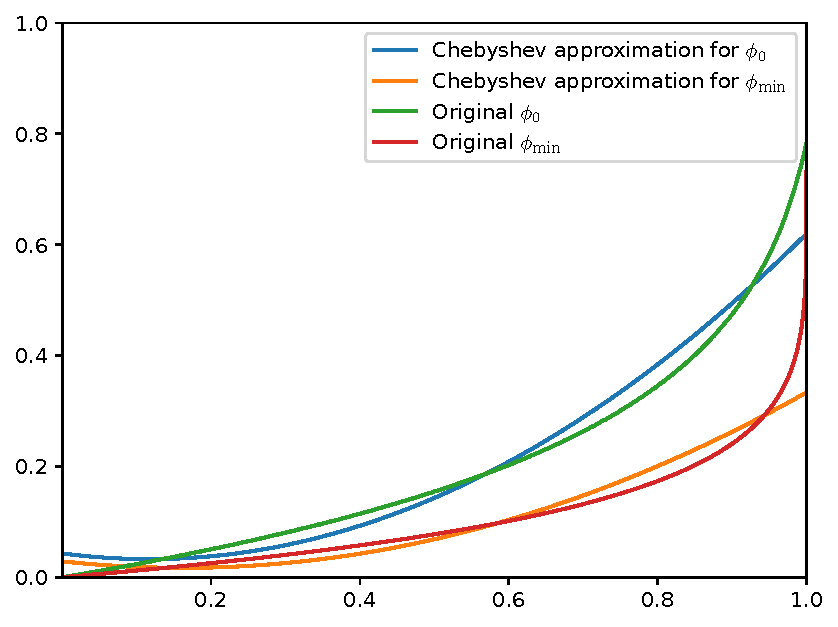
\includegraphics[scale=0.75]{plots/cheby-approx.pdf}
    \caption{Chebyshev polynomial approximations}
\end{figure}

\subsection{Attempted approximation using exponential function}

By far the most accurate fit before the original polynomial approximation, an exponential function of the form $\phi=a\exp(b(\delta-c))+d$ was used.
Significant Runge effect is still evident in the plot below.

\begin{figure}[H]
    \centering
    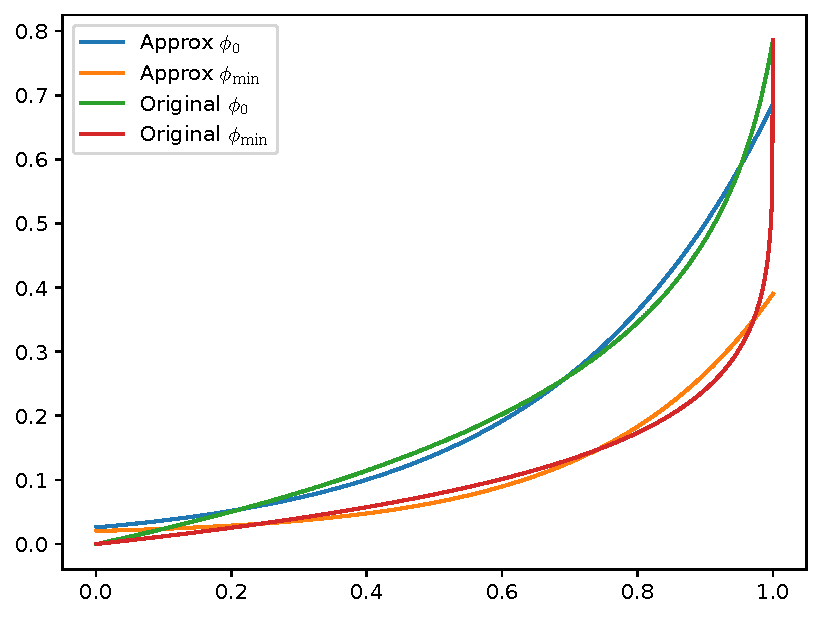
\includegraphics[scale=0.75]{plots/exponential-approx.pdf}
    \caption{Exponential approximations}
\end{figure}

\subsection{Attempted elliptical integral approximation}

Through parameterizing the first-order elliptic integral $K(k;n)$ for some $n\in \mathbb{R}$ and $k\in[0,1]$ for both translation and dilation control, curve fitting was attempted:

\begin{equation}
    K(k;n)=-\frac{\pi}{2n}+\int_0^1 \frac{dx}{n\sqrt{(1-x^2)(1-k^2x^2)}}
\end{equation}

The optimization routine returned a value of $n=1$ for both $\phi_0$ and $\phi_\mathrm{min}$, indicating that the first-order approximation is not effective. The plot is shown below.

\begin{figure}[H]
    \centering
    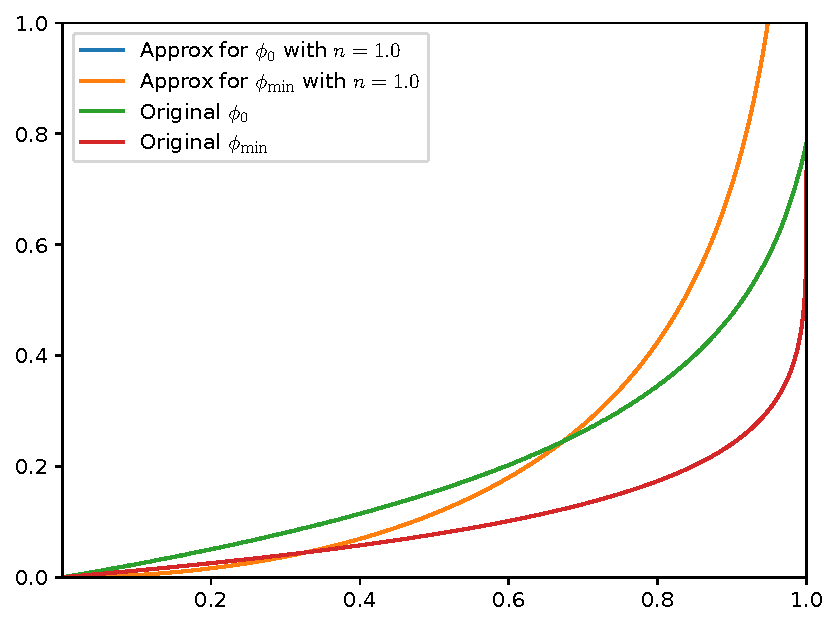
\includegraphics[scale=0.75]{plots/elliptical-approx.pdf}
    \caption{Elliptical approximations}
\end{figure}

Other possible parameterizations of the first-order functions and possibly of the higher orders will be evaluated, so this is a WIP.